\section{Funktionsweise des Ansatzes}
\label{sec:FunktionsweiseAnsatz}

In Figure \ref{fig:componentoverview} we specify the main components which build the subsystem mentioned in Section \ref{sec:systemoverview}. We highlight the components which require an extension, and the new components which are implemented and included in the system. 

\begin{figure}[htb]
	\centering
		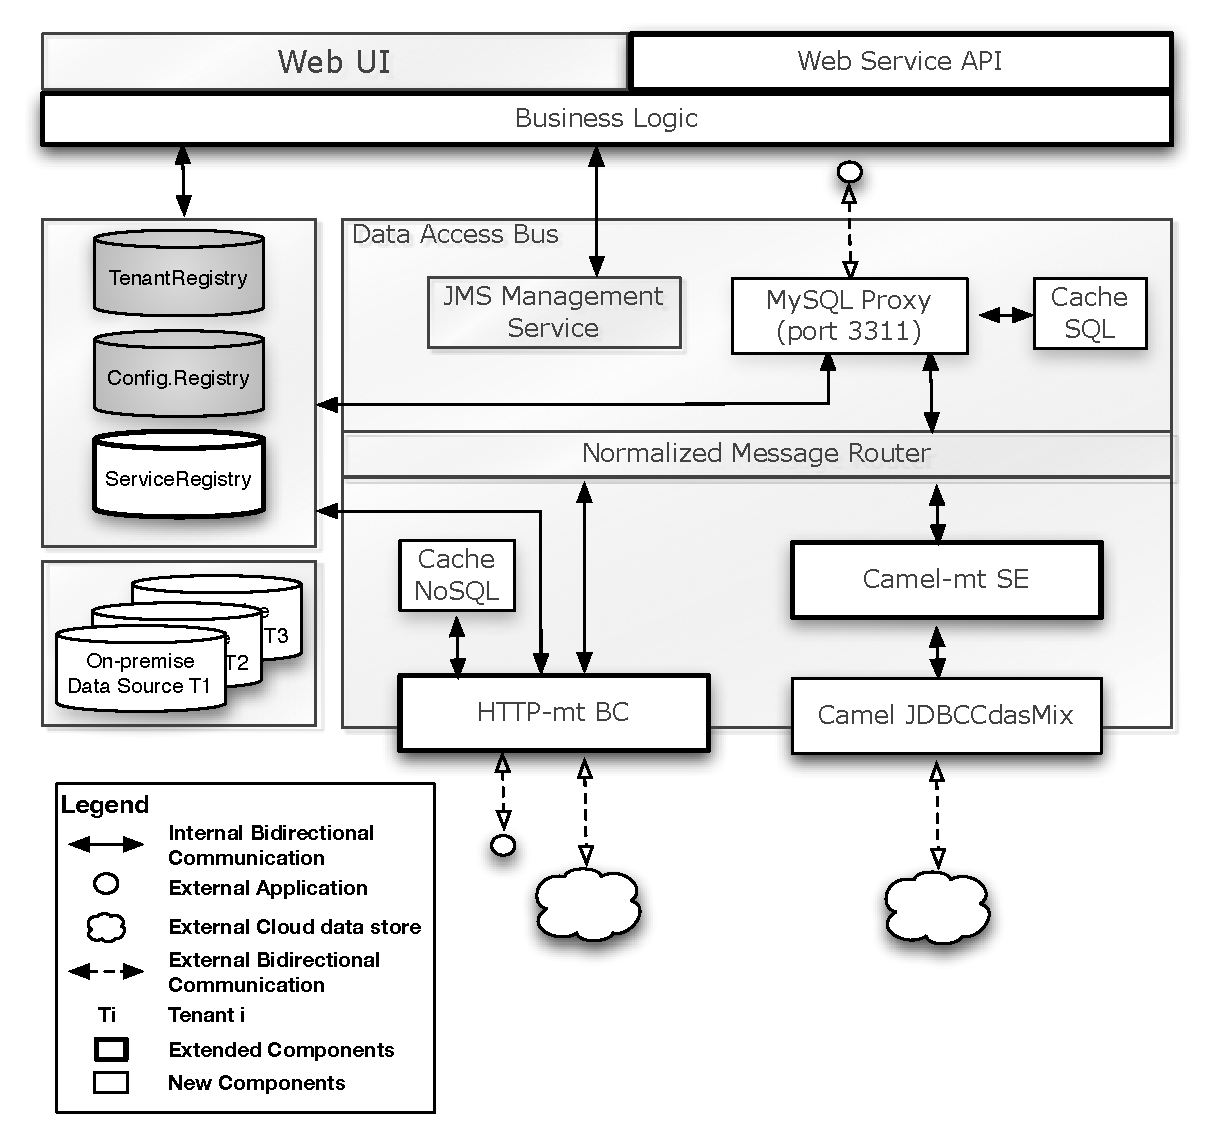
\includegraphics[clip, scale=0.6]{./gfx/componentoverview.pdf}
	\caption[Transparent Cloud Data Access Components Overview]{Transparent Cloud data access components overview.}
	\label{fig:componentoverview}
\end{figure}

As described in Section \ref{sec:systemoverview}, we extend the JBIMulti2 Web service \ac{API} and its associated business logic. The operations we include perform access and modifications to one particular registry: the Service Registry. This registry persists information about services, its policies, and \ac{SA}s deployed by one tenant. The last kind of information is the one we mainly focus on, due to the information which is contained in it: the tenant-aware endpoint configuration in ServiceMix-mt. Therefore, we extend this registry to persist the configuration about the data stores. We make a differentiation between data stores and name it source and target data sources, to be able to relate the one that the tenant physically accesses and the one which the tenant logically accesses, which is the one that the system physically accesses. To support transparent access to two different database types, we divide our architecture and implementation into the the communication protocols they support: MySQL for MySQL databases, and HTTP for \ac{NoSQL} databases (see Figure \ref{fig:componentoverview}). 

For the first one, the single access physical endpoint is provided through a \ac{TCP} port, which then forwards the message to the appropriate tenant's endpoint in the multi-tenant Servicemix Camel component, and this to the component which physically connects to the backend \ac{SQL} \ac{DBMS}. For the second one, we extend the Servicemix-http-mt in order to physically connect to the backend \ac{NoSQL} data stores. 

The possibility of migrating a database to the VM instance where the \ac{ESB} runs is also supported. However, we do not provide a multi-tenant \ac{DBMS} where a database or table is shared between multiple tenants, since it is not a requirement in this diploma thesis. The ensured isolation in this case is the one provided by a \ac{DBMS} between different databases. Furthermore, backup, restoration, administration, and horizontal scalability services are not supported. We provide in the VM instance where CDASMix runs a MySQL database system. The number and types of databases systems supported in the VM instance relies on the administrator, and the PostgreSQL database system where the system registries are stored must be independent from the PostgreSQL instance which hosts the migrated tenant's databases.

As represented in Figure \ref{fig:componentoverview}, we enhance ServiceMix-mt with cashing support, in particular for the two different types of databases we support. The cashing mechanism supports storage of access control data, as well as retrieved data from the backend data store, e.g. a bucket, or a set of rows. The reasons for using a divided cashing system instead of a single one is explained in Chapter \ref{chap:design}. 

\FloatBarrier